\documentclass[11pt,letterpaper]{article}
\usepackage{../assets/scientific_report}
\usepackage{float}
\usepackage{listings}
\usepackage{xcolor}
\usepackage{geometry}
\geometry{headheight=23pt, top=2cm, bottom=2cm, left=2.5cm, right=2.5cm}
\setlength{\parskip}{0.5em}
\setlength{\parindent}{0pt}

\lstset{
    language=C,
    basicstyle=\ttfamily\small,
    keywordstyle=\color{blue}\bfseries,
    commentstyle=\color{green!60!black}\itshape,
    stringstyle=\color{red!80!black},
    numbers=left,
    numberstyle=\tiny\color{gray},
    numbersep=8pt,
    frame=single,
    breaklines=true,
    captionpos=b,
    tabsize=4,
    showstringspaces=false
}

\begin{document}
\pagestyle{plain}

\begin{center}
    {\LARGE\bfseries Paralelismo ao Nível de Instrução (ILP)}\\[0.4em]
    {\large Dependências de dados e níveis de otimização em C}\\[1em]
    {\normalsize Eugênio Vitor Lopes dos Santos}\\[0.3em]
    {\small DCA3703 -- Programação Paralela, Universidade Federal do Rio Grande do Norte}\\[0.3em]
    {\small 2026}
\end{center}


\section{Enunciado}
Implementar três laços em C para investigar ILP: inicializar um vetor com um
cálculo simples, somar seus elementos com dependência entre iterações e repetir
a soma com múltiplos acumuladores. Comparar versões compiladas com \texttt{-O0},
\texttt{-O2} e \texttt{-O3}, analisando o efeito do estilo do código e das
dependências no desempenho.

\section{Fundamentação teórica}
ILP é a capacidade de uma CPU executar simultaneamente instruções independentes
de um mesmo fluxo. No laço dependente, cada soma precisa do resultado anterior:
\(s_{i+1}=s_i+v[i+1]\). Essa cadeia limita o número de somas que podem ser
iniciadas em paralelo. Com quatro acumuladores, as iterações são distribuídas
entre quatro cadeias independentes; o processador e o compilador podem explorar
mais ILP. O laço de inicialização não possui dependência entre
escritas diferentes, o que facilita a vetorização.

\section{Experimento}
O vetor contém \(N=100.000.000\) inteiros e é inicializado por
\texttt{v[i] = 3*i + 1}. Depois, os dois laços de soma percorrem o mesmo vetor.
Os tempos foram medidos apenas no corpo de cada laço com
\texttt{clock\_gettime(CLOCK\_MONOTONIC)}. O programa também verifica que as
duas somas produzem o mesmo resultado. Comandos de compilação:
\begin{lstlisting}[language=bash]
gcc -std=c11 -Wall -Wextra -O0 tarefa03.c -o tarefa03_O0
gcc -std=c11 -Wall -Wextra -O2 tarefa03.c -o tarefa03_O2
gcc -std=c11 -Wall -Wextra -O3 tarefa03.c -o tarefa03_O3
\end{lstlisting}

\section{Código-fonte}
\begin{lstlisting}[caption={tarefa03.c}]
#define _POSIX_C_SOURCE 199309L

#include <stdio.h>
#include <stdlib.h>
#include <time.h>

#define DEFAULT_N 100000000L

static double agora(void) {
    struct timespec t;
    clock_gettime(CLOCK_MONOTONIC, &t);
    return t.tv_sec + t.tv_nsec / 1e9;
}

int main(int argc, char **argv) {
    long n = argc > 1 ? atol(argv[1]) : DEFAULT_N;
    if (n <= 0) {
        fprintf(stderr, "Uso: %s [numero_de_elementos]\n", argv[0]);
        return 1;
    }

    int *v = malloc((size_t)n * sizeof(*v));
    if (!v) {
        perror("malloc");
        return 1;
    }

    double inicio = agora();
    for (long i = 0; i < n; ++i)
        v[i] = (int)(3 * i + 1);
    double tempo_inicializacao = agora() - inicio;

    inicio = agora();
    long long soma_dependente = 0;
    for (long i = 0; i < n; ++i)
        soma_dependente += v[i];
    double tempo_dependente = agora() - inicio;

    inicio = agora();
    long long s0 = 0, s1 = 0, s2 = 0, s3 = 0;
    long i = 0;
    for (; i + 3 < n; i += 4) {
        s0 += v[i];
        s1 += v[i + 1];
        s2 += v[i + 2];
        s3 += v[i + 3];
    }
    for (; i < n; ++i)
        s0 += v[i];
    long long soma_multiplos = s0 + s1 + s2 + s3;
    double tempo_multiplos = agora() - inicio;

    printf("N=%ld inicializacao=%.9f dependente=%.9f multiplos=%.9f "
           "somas=%lld,%lld\n", n, tempo_inicializacao,
           tempo_dependente, tempo_multiplos, soma_dependente,
           soma_multiplos);
    free(v);
    return soma_dependente != soma_multiplos;
}
\end{lstlisting}

\section{Resultados}
\begin{table}[H]
\centering
\caption{Tempo em segundos para \(N=100.000.000\).}
\begin{tabular}{lrrr}
\hline
Otimização & Inicialização & Soma dependente & Múltiplos acumuladores\\
\hline
O0 & 0,300583 & 0,151139 & 0,058475\\
O2 & 0,102487 & 0,028251 & 0,026156\\
O3 & 0,109349 & 0,026172 & 0,030444\\
\hline
\end{tabular}
\end{table}

\begin{figure}[H]
\centering
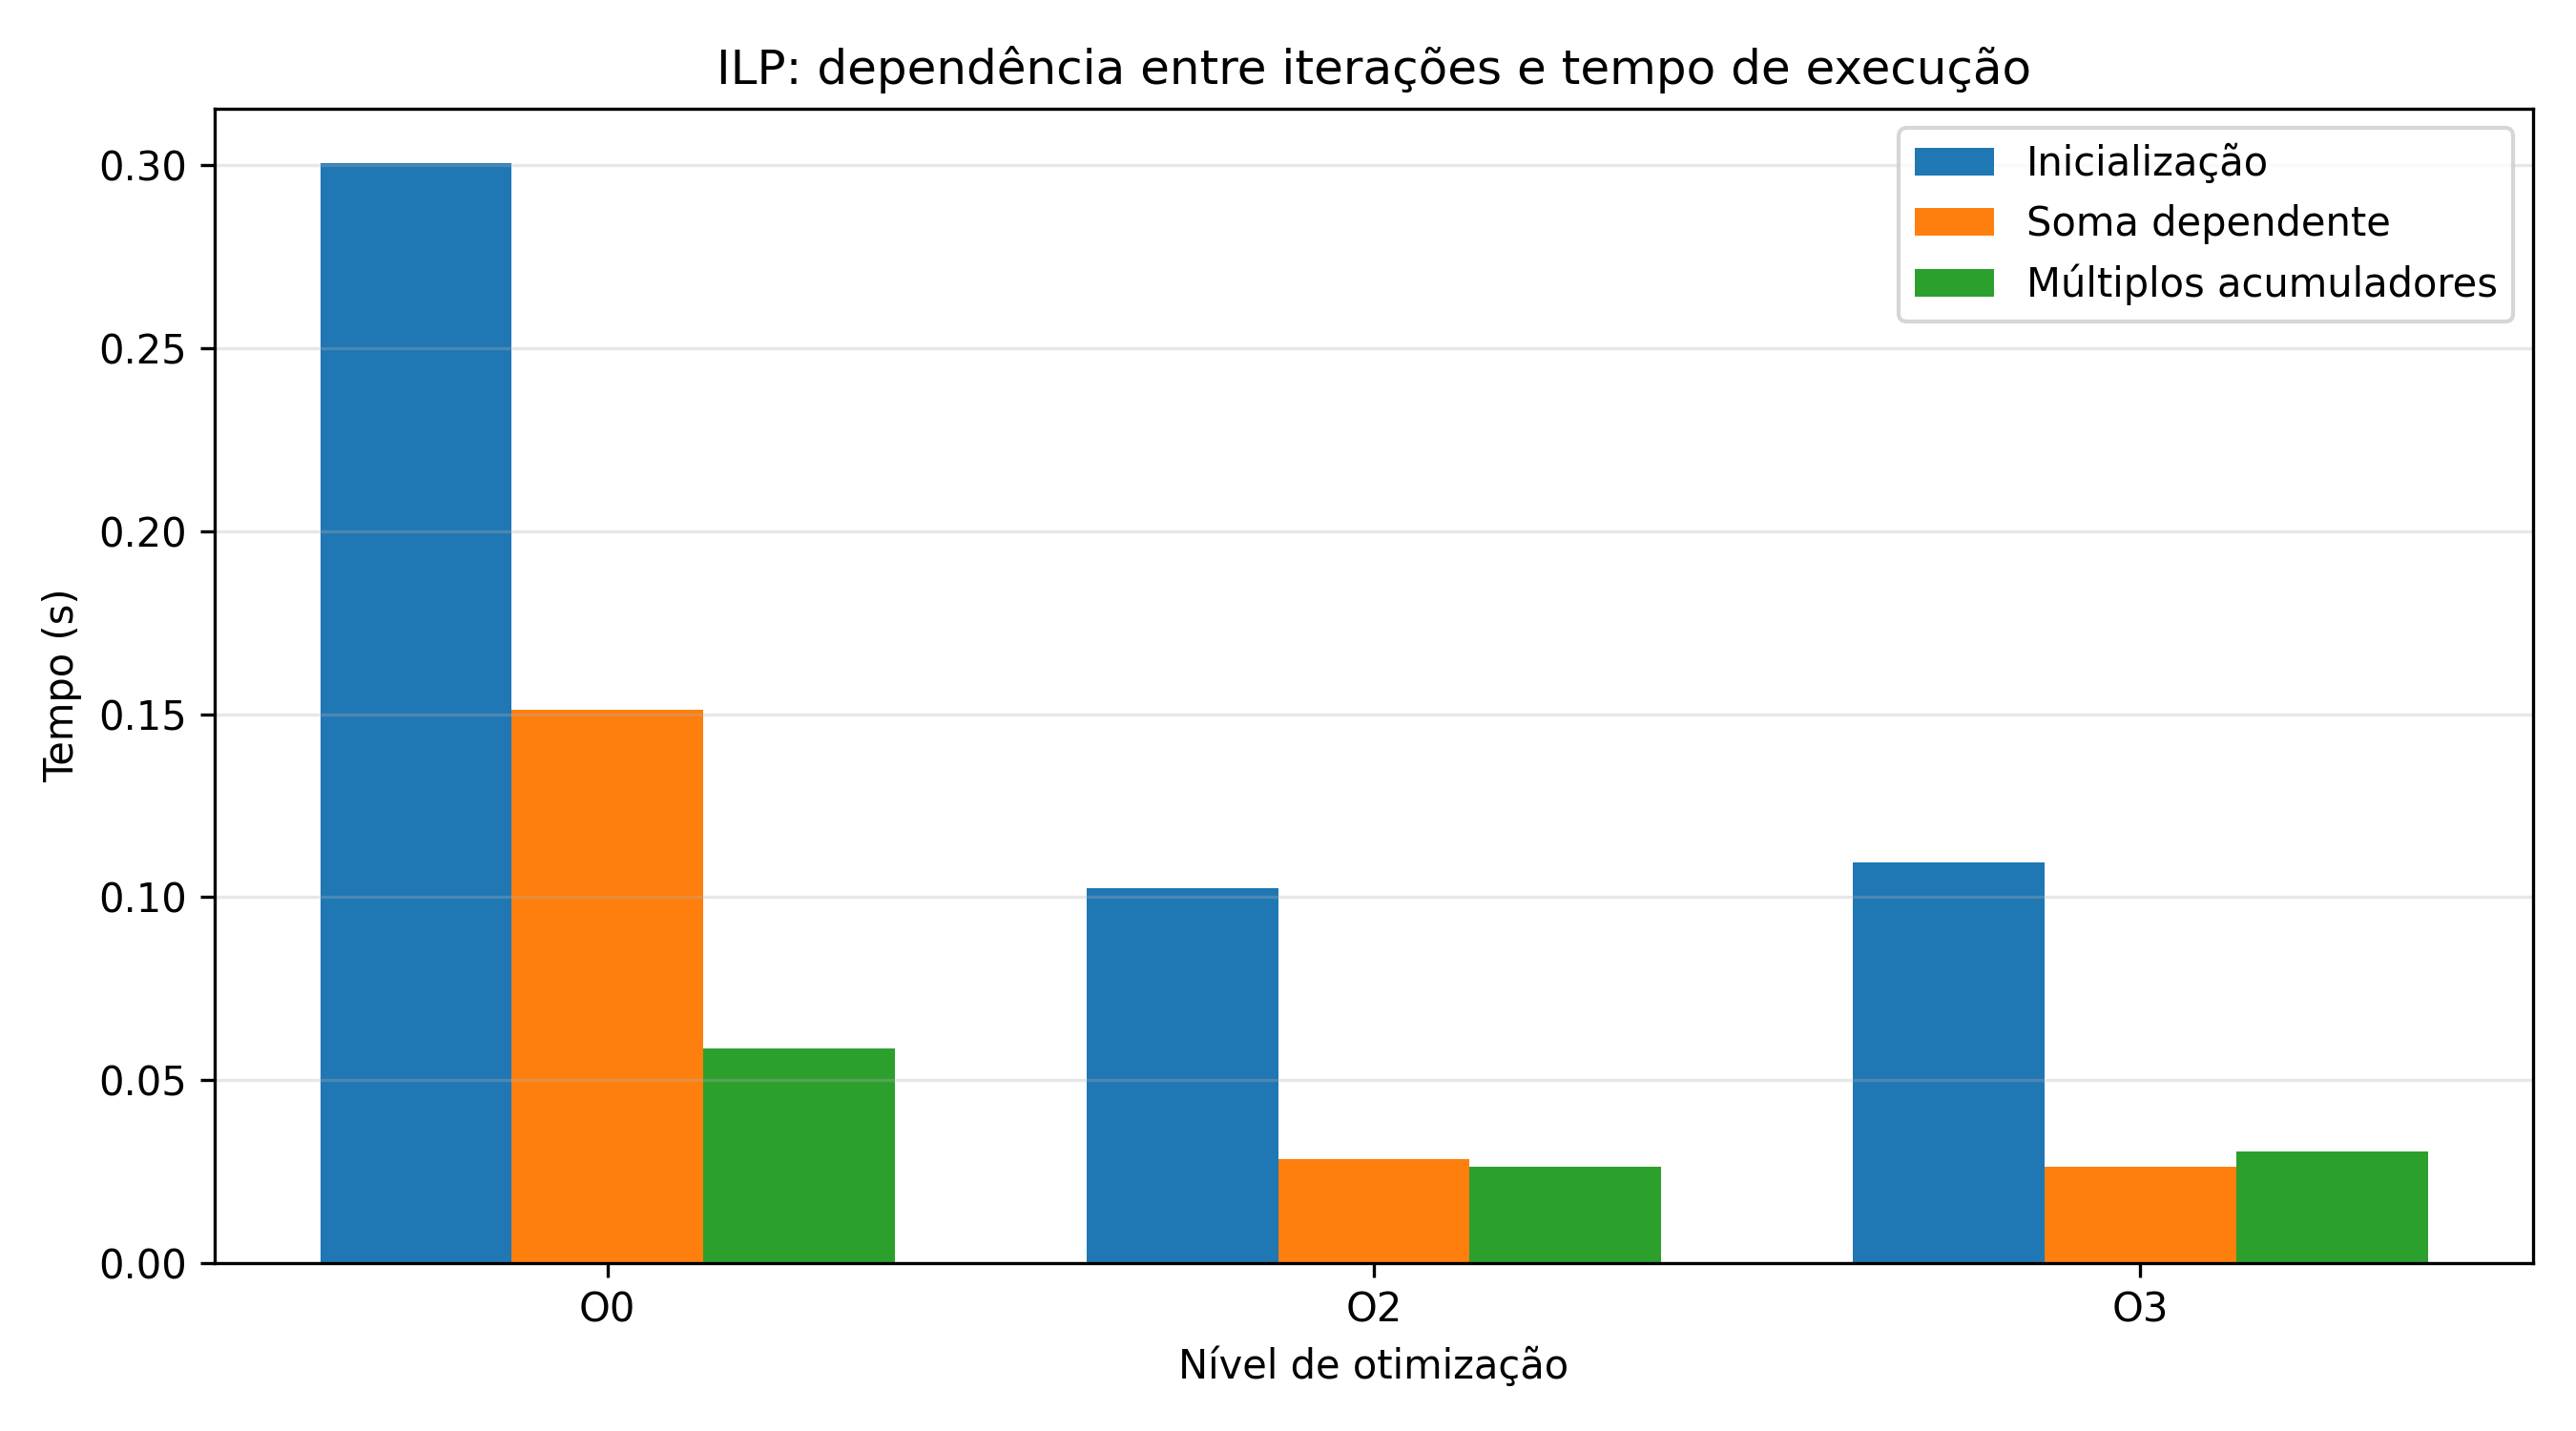
\includegraphics[width=0.9\textwidth]{ilp_results.png}
\caption{Tempo de execução dos três laços por nível de otimização ($N=100.000.000$).}
\label{fig:ilp_results}
\end{figure}

Em \texttt{-O0}, a soma com múltiplos acumuladores levou 0,058 s contra
0,151 s da soma dependente, 2,6$\times$ mais rápida, porque expõe quatro
cadeias de cálculo independentes. Em \texttt{-O2} e \texttt{-O3}, o compilador
já transforma ou vetoriza partes dos laços, e a vantagem explícita dos
acumuladores diminui. O3 não foi mais rápido que O2 no terceiro laço nesta
execução (0,030 s contra 0,026 s). A diferença é pequena e pode resultar de
ruído, frequência da CPU ou escolhas distintas de código gerado. Uma inspeção
do assembly (\texttt{gcc -S}) permitiria verificar se O3 escolheu uma
estratégia de vetorização diferente de O2, mas essa análise fica como trabalho
futuro. A inicialização caiu de 0,301 s em O0 para 0,109 s em O3.

\section{Discussão}
As três versões realizam \(O(N)\) operações, mas não apresentam o mesmo custo
constante. A dependência do acumulador único forma um caminho crítico de $N$
somas encadeadas. Os acumuladores múltiplos quebram esse caminho e permitem
sobreposição de somas. Em troca, exigem uma redução final dos quatro parciais.
Com \texttt{-O2} ou \texttt{-O3}, o compilador aplica desenrolamento e
vetorização sem alteração manual do código, e a diferença entre os estilos
diminui.

O experimento é sequencial: ILP ocorre dentro de um núcleo e não deve ser
confundido com paralelismo entre threads ou núcleos. Os tempos são de uma
execução e podem variar com carga do sistema, frequência e estado das caches.
Repetições e mediana reduziriam esse ruído.

\section{Conclusão}
O experimento mostrou que dependências entre iterações limitam o ILP. Sem
otimização, a soma com quatro acumuladores foi 2,6$\times$ mais rápida. Com O2
e O3, o compilador explorou boa parte desse paralelismo por conta própria. O
padrão de dependências afeta o tempo de execução de forma comparável à
complexidade assintótica.

\begin{thebibliography}{9}
\bibitem{hennessy2019}
J.~L.~Hennessy e D.~A.~Patterson, \textit{Computer Architecture: A Quantitative Approach}, 6ª~ed. Morgan Kaufmann, 2019.

\bibitem{intel2024}
Intel Corporation, \textit{Intel 64 and IA-32 Architectures Optimization Reference Manual}, 2024.
\end{thebibliography}

\end{document}
